\documentclass[brazil]{beamer}
%\usepackage[latin1]{inputenc}
\usepackage{beamerthemesplit}

\usepackage{graphicx,hyperref,url}
\usepackage[utf8]{inputenc}
\usepackage[T1]{fontenc}
\usepackage[portuges,brazilian]{babel}
%%%\usepackage{wrapfig}
\usepackage{caption}
\usepackage{subfigure}

\usepackage{latexsym}
\usepackage{amssymb, amsmath}
\usepackage{multicol}
\usepackage{pifont}%,bbding}%%,dingbat} %%% ver manual de simbolos
\usepackage[final]{listings}
\usepackage{comment}
\usepackage{upquote}

\usetheme{Boadilla}

\setbeamerfont{frametitle}{size=\Large}

\definecolor{editorGray}{rgb}{0.95, 0.95, 0.95}
\definecolor{editorOcher}{rgb}{1, 0.5, 0} % #FF7F00 -> rgb(239, 169, 0)
\definecolor{editorGreen}{rgb}{0, 0.5, 0} % #007C00 -> rgb(0, 124, 0)

\definecolor{cinza}{RGB}{245,245,245}
\definecolor{cinza2}{RGB}{170,170,170}
\definecolor{cinza3}{RGB}{60,60,60}
\definecolor{amareloclaro}{RGB}{255,255,230}
\definecolor{amareloescuro}{RGB}{150,150,0}
\definecolor{verdeescuro}{RGB}{0,150,0}

\definecolor{azulclaro}{rgb}{0.9,0.9,0.9}
\definecolor{mygreen}{rgb}{0,0.6,0}
\definecolor{mygray}{rgb}{0.5,0.5,0.5}
\definecolor{mymauve}{rgb}{0.58,0,0.82}
\definecolor{darkgray}{rgb}{.4,.4,.4}
\definecolor{purple}{rgb}{0.65, 0.12, 0.82}

\setbeamercolor{frametitle}{fg=blue}
\setbeamercolor{frametitle}{bg=cinza}

\setbeamercolor{section in head/foot}{fg=cinza3, bg=cinza2}



\lstdefinelanguage{JavaScript}{
      morekeywords={break, case, catch, continue, debugger, default, delete,         do, else, false, finally, for, function, if, in, instanceof, new, null, return, switch, this, throw, true, try, typeof, var, void, while, with},
      morecomment=[s]{/*}{*/},
      morecomment=[l]//,
      morestring=[b]",
      morestring=[b]'
    }
\lstdefinelanguage{CSS}{
  keywords={accelerator,azimuth,background,background-attachment,
        background-color,background-image,background-position,
        background-position-x,background-position-y,background-repeat,
        behavior,border,border-bottom,border-bottom-color,
        border-bottom-style,border-bottom-width,border-collapse,
        border-color,border-left,border-left-color,border-left-style,
        border-left-width,border-right,border-right-color,
        border-right-style,border-right-width,border-spacing,
        border-style,border-top,border-top-color,border-top-style,
        border-top-width,border-width,bottom,caption-side,clear,
        clip,color,content,counter-increment,counter-reset,cue,
        cue-after,cue-before,cursor,direction,display,elevation,
        empty-cells,filter,float,font,font-family,font-size,
        font-size-adjust,font-stretch,font-style,font-variant,
        font-weight,height,ime-mode,include-source,
        layer-background-color,layer-background-image,layout-flow,
        layout-grid,layout-grid-char,layout-grid-char-spacing,
        layout-grid-line,layout-grid-mode,layout-grid-type,left,
        letter-spacing,line-break,line-height,list-style,
        list-style-image,list-style-position,list-style-type,margin,
        margin-bottom,margin-left,margin-right,margin-top,
        marker-offset,marks,max-height,max-width,min-height,
        min-width,-moz-binding,-moz-border-radius,
        -moz-border-radius-topleft,-moz-border-radius-topright,
        -moz-border-radius-bottomright,-moz-border-radius-bottomleft,
        -moz-border-top-colors,-moz-border-right-colors,
        -moz-border-bottom-colors,-moz-border-left-colors,-moz-opacity,
        -moz-outline,-moz-outline-color,-moz-outline-style,
        -moz-outline-width,-moz-user-focus,-moz-user-input,
        -moz-user-modify,-moz-user-select,orphans,outline,
        outline-color,outline-style,outline-width,overflow,
        overflow-X,overflow-Y,padding,padding-bottom,padding-left,
        padding-right,padding-top,page,page-break-after,
        page-break-before,page-break-inside,pause,pause-after,
        pause-before,pitch,pitch-range,play-during,position,quotes,
        -replace,richness,right,ruby-align,ruby-overhang,
        ruby-position,-set-link-source,size,speak,speak-header,
        speak-numeral,speak-punctuation,speech-rate,stress,
        scrollbar-arrow-color,scrollbar-base-color,
        scrollbar-dark-shadow-color,scrollbar-face-color,
        scrollbar-highlight-color,scrollbar-shadow-color,
        scrollbar-3d-light-color,scrollbar-track-color,table-layout,
        text-align,text-align-last,text-decoration,text-indent,
        text-justify,text-overflow,text-shadow,text-transform,
        text-autospace,text-kashida-space,text-underline-position,top,
        unicode-bidi,-use-link-source,vertical-align,visibility,
        voice-family,volume,white-space,widows,width,word-break,
        word-spacing,word-wrap,writing-mode,z-index,zoom},  
  sensitive=true,
  morecomment=[l]{//},
  morecomment=[s]{/*}{*/},
  morestring=[b]',
  morestring=[b]",
  alsoletter={:},
  alsodigit={-}
}
\lstdefinelanguage{HTML5}{
        language=html,
        sensitive=true, 
        alsoletter={<>=-},
        otherkeywords={
        % HTML tags
        <, </, >,
        </a, <a, </a>,
        </abbr, <abbr, </abbr>,
        </address, <address, </address>,
        </area, <area, </area>,
        </area, <area, </area>,
        </article, <article, </article>,
        </aside, <aside, </aside>,
        </audio, <audio, </audio>,
        </audio, <audio, </audio>,
        </b, <b, </b>,
        </base, <base, </base>,
        </bdi, <bdi, </bdi>,
        </bdo, <bdo, </bdo>,
        </blockquote, <blockquote, </blockquote>,
        </body, <body, </body>,
        </br, <br, </br>,
        </button, <button, </button>,
        </canvas, <canvas, </canvas>,
        </caption, <caption, </caption>,
        </cite, <cite, </cite>,
        </code, <code, </code>,
        </col, <col, </col>,
        </colgroup, <colgroup, </colgroup>,
        </data, <data, </data>,
        </datalist, <datalist, </datalist>,
        </dd, <dd, </dd>,
        </del, <del, </del>,
        </details, <details, </details>,
        </dfn, <dfn, </dfn>,
        </div, <div, </div>,
        </dl, <dl, </dl>,
        </dt, <dt, </dt>,
        </em, <em, </em>,
        </embed, <embed, </embed>,
        </fieldset, <fieldset, </fieldset>,
        </figcaption, <figcaption, </figcaption>,
        </figure, <figure, </figure>,
        </footer, <footer, </footer>,
        </form, <form, </form>,
        </h1, <h1, </h1>,
        </h2, <h2, </h2>,
        </h3, <h3, </h3>,
        </h4, <h4, </h4>,
        </h5, <h5, </h5>,
        </h6, <h6, </h6>,
        </head, <head, </head>,
        </header, <header, </header>,
        </hr, <hr, </hr>,
        </html, <html, </html>,
        </i, <i, </i>,
        </iframe, <iframe, </iframe>,
        </img, <img, </img>,
        </input, <input, </input>,
        </ins, <ins, </ins>,
        </kbd, <kbd, </kbd>,
        </keygen, <keygen, </keygen>,
        </label, <label, </label>,
        </legend, <legend, </legend>,
        </li, <li, </li>,
        </link, <link, </link>,
        </main, <main, </main>,
        </map, <map, </map>,
        </mark, <mark, </mark>,
        </math, <math, </math>,
        </menu, <menu, </menu>,
        </menuitem, <menuitem, </menuitem>,
        </meta, <meta, </meta>,
        </meter, <meter, </meter>,
        </nav, <nav, </nav>,
        </noscript, <noscript, </noscript>,
        </object, <object, </object>,
        </ol, <ol, </ol>,
        </optgroup, <optgroup, </optgroup>,
        </option, <option, </option>,
        </output, <output, </output>,
        </p, <p, </p>,
        </param, <param, </param>,
        </pre, <pre, </pre>,
        </progress, <progress, </progress>,
        </q, <q, </q>,
        </rp, <rp, </rp>,
        </rt, <rt, </rt>,
        </ruby, <ruby, </ruby>,
        </s, <s, </s>,
        </samp, <samp, </samp>,
        </script, <script, </script>,
        </section, <section, </section>,
        </select, <select, </select>,
        </small, <small, </small>,
        </source, <source, </source>,
        </span, <span, </span>,
        </strong, <strong, </strong>,
        </style, <style, </style>,
        </summary, <summary, </summary>,
        </sup, <sup, </sup>,
        </svg, <svg, </svg>,
        </table, <table, </table>,
        </tbody, <tbody, </tbody>,
        </td, <td, </td>,
        </template, <template, </template>,
        </textarea, <textarea, </textarea>,
        </tfoot, <tfoot, </tfoot>,
        </th, <th, </th>,
        </thead, <thead, </thead>,
        </time, <time, </time>,
        </title, <title, </title>,
        </tr, <tr, </tr>,
        </track, <track, </track>,
        </u, <u, </u>,
        </ul, <ul, </ul>,
        </var, <var, </var>,
        </video, <video, </video>,
        </wbr, <wbr, </wbr>,
        />, <!
        },  
        ndkeywords={
        % General
        =,
        % HTML attributes
        accept=, accept-charset=, accesskey=, action=, align=, alt=, async=, autocomplete=, autofocus=, autoplay=, autosave=, bgcolor=, border=, buffered=, challenge=, charset=, checked=, cite=, class=, code=, codebase=, color=, cols=, colspan=, content=, contenteditable=, contextmenu=, controls=, coords=, data=, datetime=, default=, defer=, dir=, dirname=, disabled=, download=, draggable=, dropzone=, enctype=, for=, form=, formaction=, headers=, height=, hidden=, high=, href=, hreflang=, http-equiv=, icon=, id=, ismap=, itemprop=, keytype=, kind=, label=, lang=, language=, list=, loop=, low=, manifest=, max=, maxlength=, media=, method=, min=, multiple=, name=, novalidate=, open=, optimum=, pattern=, ping=, placeholder=, poster=, preload=, pubdate=, radiogroup=, readonly=, rel=, required=, reversed=, rows=, rowspan=, sandbox=, scope=, scoped=, seamless=, selected=, shape=, size=, sizes=, span=, spellcheck=, src=, srcdoc=, srclang=, start=, step=, style=, summary=, tabindex=, target=, title=, type=, usemap=, value=, width=, wrap=,
        % CSS properties
        accelerator:,azimuth:,background:,background-attachment:,
        background-color:,background-image:,background-position:,
        background-position-x:,background-position-y:,background-repeat:,
        behavior:,border:,border-bottom:,border-bottom-color:,
        border-bottom-style:,border-bottom-width:,border-collapse:,
        border-color:,border-left:,border-left-color:,border-left-style:,
        border-left-width:,border-right:,border-right-color:,
        border-right-style:,border-right-width:,border-spacing:,
        border-style:,border-top:,border-top-color:,border-top-style:,
        border-top-width:,border-width:,bottom:,caption-side:,clear:,
        clip:,color:,content:,counter-increment:,counter-reset:,cue:,
        cue-after:,cue-before:,cursor:,direction:,display:,elevation:,
        empty-cells:,filter:,float:,font:,font-family:,font-size:,
        font-size-adjust:,font-stretch:,font-style:,font-variant:,
        font-weight:,height:,ime-mode:,include-source:,
        layer-background-color:,layer-background-image:,layout-flow:,
        layout-grid:,layout-grid-char:,layout-grid-char-spacing:,
        layout-grid-line:,layout-grid-mode:,layout-grid-type:,left:,
        letter-spacing:,line-break:,line-height:,list-style:,
        list-style-image:,list-style-position:,list-style-type:,margin:,
        margin-bottom:,margin-left:,margin-right:,margin-top:,
        marker-offset:,marks:,max-height:,max-width:,min-height:,
        min-width:,transition-duration:,transition-property:,
        transition-timing-function:,transform:,
        -moz-transform:,-moz-binding:,-moz-border-radius:,
        -moz-border-radius-topleft:,-moz-border-radius-topright:,
        -moz-border-radius-bottomright:,-moz-border-radius-bottomleft:,
        -moz-border-top-colors:,-moz-border-right-colors:,
        -moz-border-bottom-colors:,-moz-border-left-colors:,-moz-opacity:,
        -moz-outline:,-moz-outline-color:,-moz-outline-style:,
        -moz-outline-width:,-moz-user-focus:,-moz-user-input:,
        -moz-user-modify:,-moz-user-select:,orphans:,outline:,
        outline-color:,outline-style:,outline-width:,overflow:,
        overflow-X:,overflow-Y:,padding:,padding-bottom:,padding-left:,
        padding-right:,padding-top:,page:,page-break-after:,
        page-break-before:,page-break-inside:,pause:,pause-after:,
        pause-before:,pitch:,pitch-range:,play-during:,position:,quotes:,
        -replace:,richness:,right:,ruby-align:,ruby-overhang:,
        ruby-position:,-set-link-source:,size:,speak:,speak-header:,
        speak-numeral:,speak-punctuation:,speech-rate:,stress:,
        scrollbar-arrow-color:,scrollbar-base-color:,
        scrollbar-dark-shadow-color:,scrollbar-face-color:,
        scrollbar-highlight-color:,scrollbar-shadow-color:,
        scrollbar-3d-light-color:,scrollbar-track-color:,table-layout:,
        text-align:,text-align-last:,text-decoration:,text-indent:,
        text-justify:,text-overflow:,text-shadow:,text-transform:,
        text-autospace:,text-kashida-space:,text-underline-position:,top:,
        unicode-bidi:,-use-link-source:,vertical-align:,visibility:,
        voice-family:,volume:,white-space:,widows:,width:,word-break:,
        word-spacing:,word-wrap:,writing-mode:,z-index:,zoom:
        },  
        morecomment=[s]{<!--}{-->},
        tag=[s]
}



\makeatletter
\setbeamertemplate{footline}
{
  \leavevmode%
  \hbox{%
  \begin{beamercolorbox}[wd=.3\paperwidth,ht=2.25ex,dp=1ex,center]{section in head/foot}%
    \usebeamerfont{author in head/foot}{\tt \insertshortauthor~~\beamer@ifempty{\insertshortinstitute}{}{(\insertshortinstitute)}}
  \end{beamercolorbox}%
  \begin{beamercolorbox}[wd=.4\paperwidth,ht=2.25ex,dp=1ex,center]{section in head/foot}%
    \usebeamerfont{title in head/foot}{\tt \insertshorttitle}
  \end{beamercolorbox}%
  \begin{beamercolorbox}[wd=.3\paperwidth,ht=2.25ex,dp=1ex,right]{section in head/foot}%
    \usebeamerfont{date in head/foot}{\tt \insertshortdate{}}\hspace*{2em}
    {\color{black} \insertframenumber{} / \inserttotalframenumber\hspace*{2ex} }
  \end{beamercolorbox}}%
  \vskip0pt%
}
\makeatother


\newcommand{\minizinc}{MiniZinc}

%\lstset{ 
  %%  label={pgm_ex01},r
    %backgroundcolor=\color{amareloclaro}, 
    %language=erlang, %%Miranda,%%Perl,%%%Python, %%Mercury, %%C,
    %showstringspaces=false,
    %%basicstyle=\bf\scriptsize\ttfamily,
    %basicstyle=\scriptsize\ttfamily,
%%%      basicstyle= \footnotesize %%% TESTAR
%%%      keywordstyle=\bfseries\color{green!40!black},
    %keywordstyle=\textbf{\color{mygreen}}, 
    %%otherkeywords={*, \%, array, constraint, solve, output,  show, "/\", satisfy, set, of, if, then, elseif, float, search},
%%%  keywordstyle=\color{blue},       % keyword style
%%%    commentstyle=\itshape\color{purple!40!black},
      %commentstyle=\color{orange},    % comment style
      %%identifierstyle=\color{blue},
      %identifierstyle=\color{black},
      %%stringstyle=\color{orange},
      %stringstyle=\color{verdeescuro},
      %numbers=left,  % where to put the line-numbers; possible values are (none, left, right)
      %numbersep=2pt,   % how far the line-numbers are from the code
      %numberstyle=\tiny\ttfamily\color{amareloescuro},
      %keepspaces=true      
    %% %caption={LEGENDA no source PASCAL ficou OK},
%}



\lstset{%
    % Basic design
    backgroundcolor=\color{editorGray},
    basicstyle={\tiny\ttfamily},   
    frame=l,
    % Line numbers
    xleftmargin={0.75cm},
    numbers=left,
    stepnumber=1,
    firstnumber=1,
    numberfirstline=true,
    % Code design   
    keywordstyle=\color{blue}\bfseries,
    commentstyle=\color{darkgray}\ttfamily,
    ndkeywordstyle=\color{editorGreen}\bfseries,
    stringstyle=\color{editorOcher},
    % Code
    language=HTML5,
    alsodigit={.:;},
    tabsize=2,
    showtabs=false,
    showspaces=false,
    showstringspaces=false,
    extendedchars=true,
    breaklines=true,        
}



\graphicspath{{/home/ccs/Dropbox/figs_genericas/}{figuras/}{/home/ccs/Dropbox/CCS/picat/}}
\DeclareGraphicsExtensions{.pdf,.png,.jpg}
%Global Background must be put in preamble
%\usebackgroundtemplate{\includegraphics[width=\paperwidth]{amarelinho.pdf}}
%%% \begin{frame}[allowframebreaks=0.8]

% The log drawn in the upper right corner.

%\logo{\centering
%\includegraphics[height=0.050\paperheight]{figuras/logo_SBPO_Peixe.png}
%%\hspace{9.6cm}
%\includegraphics[height=0.027\paperheight]{figuras/logo_udesc_horizontal.jpg}


%%%%%%%%%%%%%%%%%%%%%%%%%%%%%%%%%%%%%%%%%%%%%%%%%%%%%%%%%%%%%%%%%%%%%


\title[Picat]{\fontsize{15}{20}\selectfont \textcolor{black}{Um Ambiente (\textit{on-line}) de Programação  para Linguagem PICAT}}

%\title{Aplicações de PDI (INE5401)}
%\author{Alexandre Gonçalves Silva\inst{1} \and 
%Claudio Cesar de Sá \inst{2} \and 
%Lucas Hermman Negri \inst{3}}
\author{A.G. Silva\inst{1} \and 
C.C. de Sá\inst{2} \and 
L.H. Negri\inst{3}}
\institute{\inst{1} Departamento Informática e Estatística -- Universidade Federal de Santa Catarina -- UFSC 
\and
\inst{2} Departamento de Ciência da Computação -- Universidade do Estado de Santa Catarina -- UDESC
\and
\inst{3}Instituto Federal de Educação, Ciência e Tecnologia de Mato Grosso do Sul -- IFMS}
\date{\today}

%%%%%%%%%%%%%%%%%%%%%%%%%%%%%%%%%%%%%%%%%%%%%%%%%%%%%%%%%%%%%%%%%%%%%
\begin{comment}
\author{Alexandre Gonçalves Silva\footnote{Departamento Informática e Estatística -- Universidade Federal de Santa Catarina -- UFSC}, Claudio Cesar de Sá\footnote{Departamento de Ciência da Computação -- Universidade do Estado de Santa Catarina -- UDESC}, Lucas Hermman Negri\footnote{Instituto Federal de Educação, Ciência e Tecnologia de Mato Grosso do Sul -- IFMS}}
\end{comment}



\begin{document}

\begin{frame}
    \titlepage
\end{frame}

%%%%%%%%%%%%%%%%%%%%%%%%%%%%%%%%%%%%%%%%%%%%%%%%%%%%%%%%%%%%%%%%%%%%%

\begin{frame}[fragile]
\frametitle{Sumário da Apresentação}
\tableofcontents
\end{frame}



%%%%%%%%%%%%%%%%%%%%%%%%%%%%%%%%%%%%%%%%%%%%%%%%%%%%%%%%%%%%%%
\section{Objetivos}


%-------------------------------------------------------------
\begin{frame}

    \frametitle{Objetivos do Trabalho}

    \begin{itemize}
      \item Apresentar a Linguagem PICAT \\~\\
      \item PICAT e suas contribuições \\~\\
      \item Finalmene, um  ambiente WEB de programação para PICAT \\~\\
    \item Conclusões
    \end{itemize}
\end{frame}


%-------------------------------------------------------------
\section{Introdução}
\begin{frame}

    \frametitle{Histórico}

    \begin{itemize}
      \item Criada em 2013 por Neng-Fa Zhou e Jonathan Fruhman \\~\\

      \item Utiliza B-Prolog como base de implementação, e ambas utilizam 
      a programação em lógica (Lógica de Primeira Ordem) \\~\\

      \item Uma evolução do Prolog após mais de 40 anos \\~\\

      \item Sua atual versão é a 2.2 (visitado em \today) \\~\\

      \item Seu sítio: \url{http://picat-lang.org/} \\~\\
      
      \item Uma \textbf{linguagem multiparadigma}
    \end{itemize}
\end{frame}
%%%%%%%%%%%%%%%%%%%%%%%%%%%%%%%%%%%%%%%%%%%%%%%%%%%%%%%%%%%%%%
\section{Características de PICAT}

\begin{frame}
    \frametitle{O que é multiparadigma?}

    \begin{itemize}
      \item Imperativo -- Procedural \\~\\
      \item Funcional \\~\\
      \item \underline{Lógico} \\~\\
      \item Uma boa \textit{mistura} de: Haskell, Prolog e Python

    \end{itemize}

\end{frame}
%-------------------------------------------------------------
\begin{frame}
    \frametitle{Algumas Características:}

    \begin{itemize}
    
      \item Sintaxe $\Rightarrow $ elegância do código \\~\\
      \item Velocidade de execução \\~\\
      \item Portabilidade (todas plataformas) \\~\\
      \item Extensão há outras ferramentas
      
    \end{itemize}
\end{frame}
%-------------------------------------------------------------
\begin{frame}
    \frametitle{Anacrônico de \textbf{P.I.C.A.T.}}
  
 \begin{description}
   
 
 \item [\textbf{P}:] \textit{Pattern-matching}:  Utiliza o conceito de \textit{casamento padrão}
 equivalente aos conceitos de \textit{unificação} da LPO
 
 \item [\textbf{I}:] \textit{Intuitive}: oferece estruturas de decisão, atribuição e 
 laços de repetição, etc, análogo as outras linguagens de programação
\item [\textbf{C}:] \textit{Constraints}: suporta a Programação por Restrições (PR)
 
     \item [\textbf{A}:] \textit{Actors}: suporte as chamadas a eventos, os atores (futuro gráfico) 
 
  \item [\textbf{T}:] \textit{Tabling}: implementa a técnica de \textit{memoization}, com soluções imediatas para problemas de Programação Dinâmica (PD).
   
  
\end{description}
\end{frame}


%%%%%%%%%%%%%%%%%%%%%%%%%%%%%%%%%%%%%%%%%%%%%%%%%%%%%%%%%%%%%%
\section{WebIDE}

%-------------------------------------------------------------
\begin{frame}

    \frametitle{Ambiente}

    \begin{itemize}
      \item Criado no primeiro semestre de 2017 \\
      \begin{itemize}
        \item \url{http://picat.retina.ufsc.br/picat.html}
      \end{itemize}

    \end{itemize}

\begin{center}
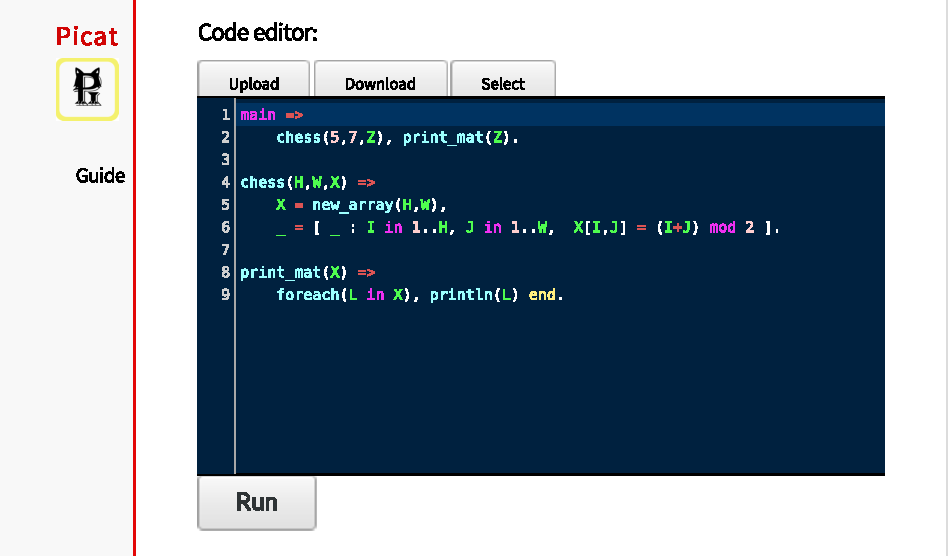
\includegraphics[width=.8\textwidth]{figures/ambiente.pdf}
\end{center}

\end{frame}




%-------------------------------------------------------------
\begin{frame}

    \frametitle{Ambiente}

    \begin{itemize}
      \item Utiliza CSS/Javascript \textbf{CodeMirror} para realce de sintaxe (\textit{syntax highlighting}), endentação e outras formatações
      \begin{itemize}
        \item \url{http://codemirror.net/}
      \end{itemize} ~\\

      \item Utiliza \textbf{Python} 2.X para uso de CGI (\textit{Common Gateway Interface}), análise preliminar de código-fonte e proteção do servidor (\textit{sandbox})
      \begin{itemize}
        \item \url{https://www.python.org/}
      \end{itemize} ~\\

      \item Utiliza \textbf{Picat} 2.2 para execução dos scripts
      \begin{itemize}
        \item \url{http://picat-lang.org/}
      \end{itemize}

    \end{itemize}
\end{frame}


%-------------------------------------------------------------
\begin{frame}

    \frametitle{\textit{Upload}}

    \begin{itemize}
      \item Interface
    \end{itemize}

\begin{center}
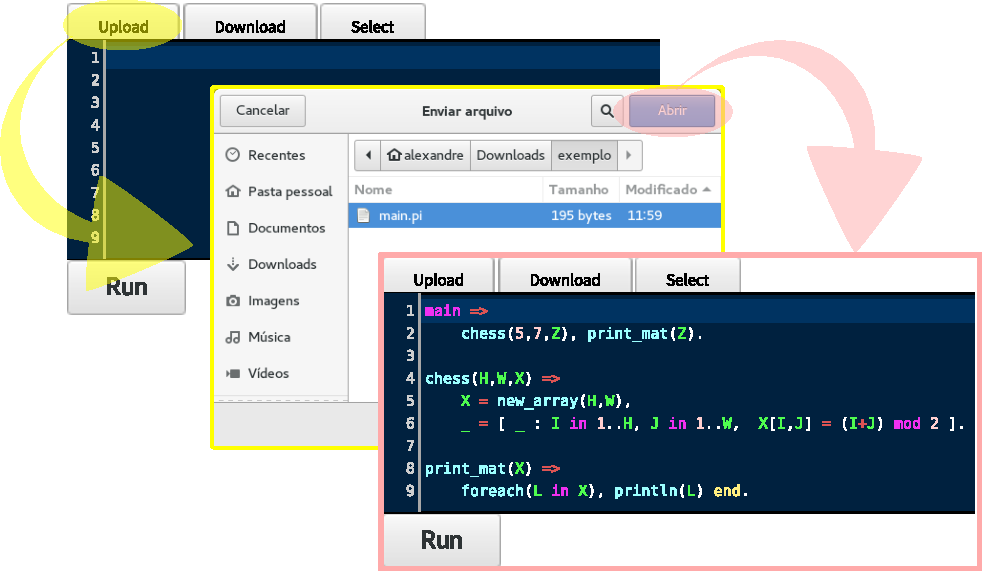
\includegraphics[width=.8\textwidth]{figures/func-upload.pdf}
\end{center}

\end{frame}


%-------------------------------------------------------------
\begin{frame}[fragile]

    \frametitle{\textit{Upload}}

    \begin{itemize}
      \item Código
    \end{itemize}

\begin{lstlisting}
<label for="upload-file">Upload</label><input type="file" onchange="loadfile(this)" id="upload-file" style="display:none">

<script>
    var editor = CodeMirror.fromTextArea(document.getElementById("code"), {
        lineNumbers: true,
        styleActiveLine: true,
        matchBrackets: true,
        extraKeys: {"Tab":  "indentAuto"},
        theme: "erlang-dark"
    });

    function loadfile(input) {
        var reader = new FileReader();
        reader.onload = function(e) {
            document.getElementById('code').value = e.target.result;
            editor.setValue(e.target.result);
        }
        reader.readAsText(input.files[0]);
    }
</script>
\end{lstlisting}

\end{frame}


%-------------------------------------------------------------
\begin{frame}

    \frametitle{\textit{Download}}

    \begin{itemize}
      \item Interface
    \end{itemize}

\begin{center}
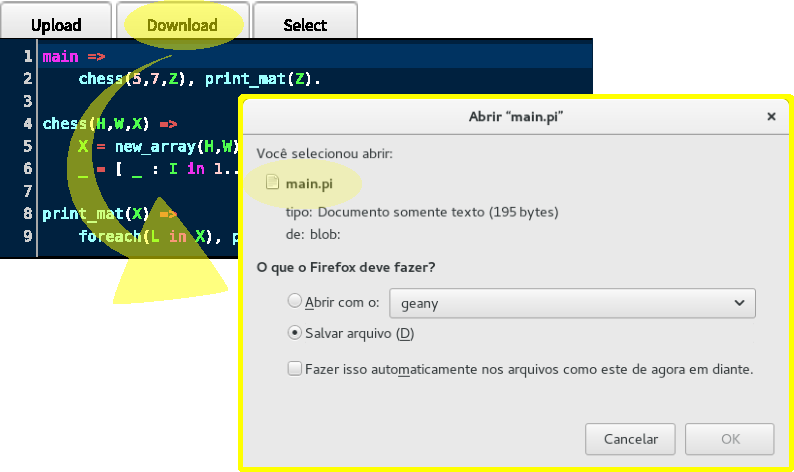
\includegraphics[width=.8\textwidth]{figures/func-download.pdf}
\end{center}

\end{frame}


%-------------------------------------------------------------
\begin{frame}[fragile]

    \frametitle{\textit{Download}}

    \begin{itemize}
      \item Código
    \end{itemize}

\begin{lstlisting}
<label for="download-file">Download</label><input onclick="saveTextAsFile()" id="download-file" style="display:none">

<script>
    function saveTextAsFile() {
        var textToWrite = document.getElementById("code").value;
        var textFileAsBlob = new Blob([textToWrite], {type:"text/plain;charset=utf-8"});
        var fileNameToSaveAs = "main.pi";

        var downloadLink = document.createElement("a");
        downloadLink.download = fileNameToSaveAs;
        downloadLink.innerHTML = "Download File";
        if (window.webkitURL != null) {
            downloadLink.href = window.webkitURL.createObjectURL(textFileAsBlob);
        }
        else {
            downloadLink.href = window.URL.createObjectURL(textFileAsBlob);
            downloadLink.onclick = destroyClickedElement;
            downloadLink.style.display = "none";
            document.body.appendChild(downloadLink);
        }

        downloadLink.click();
    }
</script>
\end{lstlisting}

\end{frame}



%-------------------------------------------------------------
\begin{frame}

    \frametitle{\textit{Select}}

    \begin{itemize}
      \item Interface
    \end{itemize}

\begin{center}
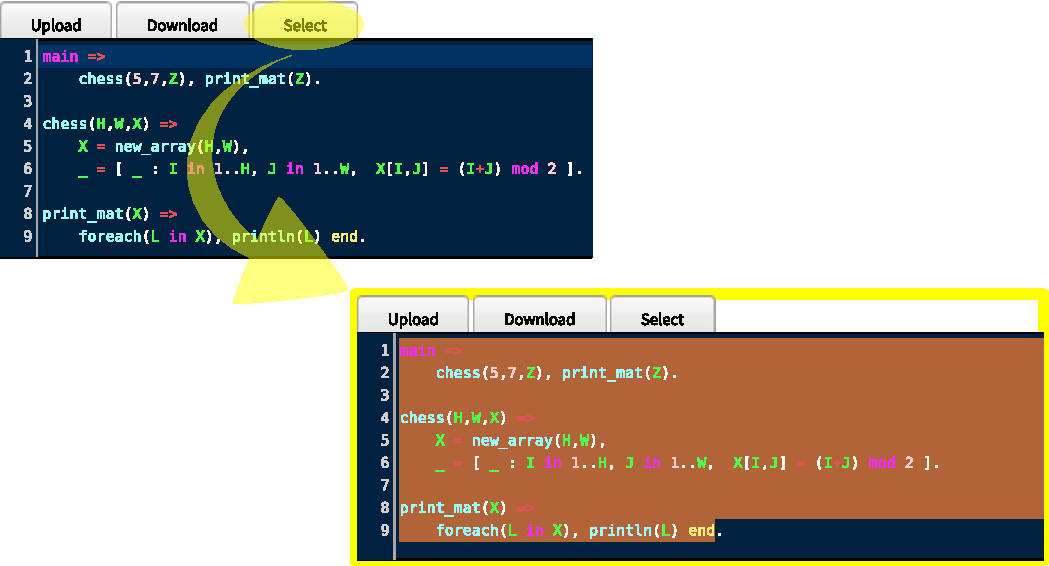
\includegraphics[width=.8\textwidth]{figures/func-select.pdf}
\end{center}

\end{frame}


%-------------------------------------------------------------
\begin{frame}[fragile]

    \frametitle{\textit{Select}}

    \begin{itemize}
      \item Código
    \end{itemize}

\begin{lstlisting}
<label for="select-file">Select</label><input onclick="mySelectAll()" id="select-file" style="display:none">

<script>
    function mySelectAll() {
        editor.execCommand("selectAll");
        document.execCommand("copy");
    }
</script>
\end{lstlisting}

\end{frame}



%-------------------------------------------------------------
\begin{frame}

    \frametitle{\textit{Run}}

    \begin{itemize}
      \item Funcionamento
    \end{itemize}

\begin{center}
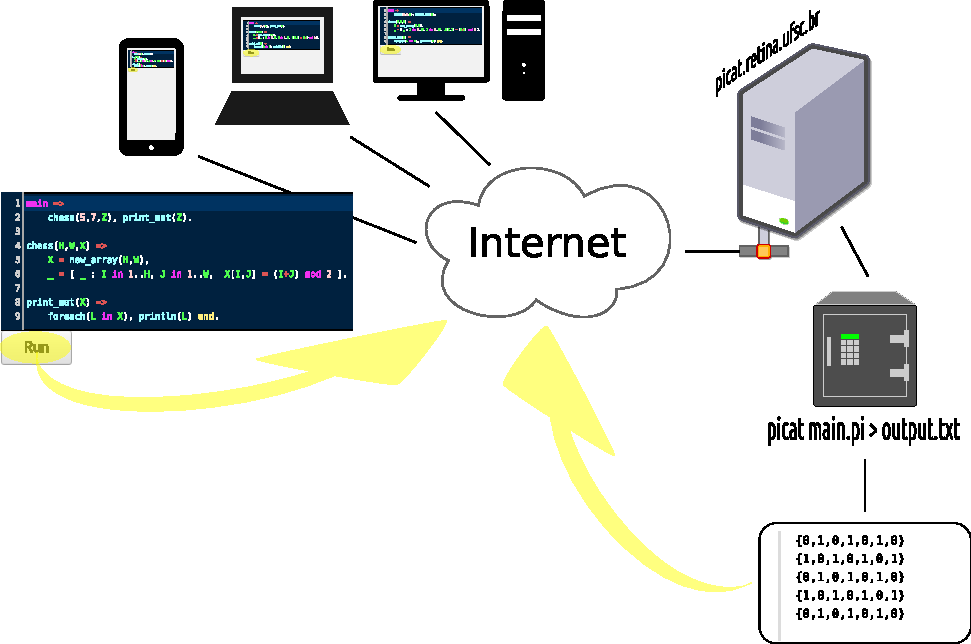
\includegraphics[width=.8\textwidth]{figures/func-run.pdf}
\end{center}

\end{frame}


%-------------------------------------------------------------
\begin{frame}[fragile]

    \frametitle{\textit{Run}}

    \begin{itemize}
      \item Código para execução do script Picat
    \end{itemize}

\begin{lstlisting}[language=Python]
    if re.findall('import\s*os', codepi) or re.findall('command\s*\(', codepi) or re.findall('apply\s*\(', codepi):
        codeout = 'Module "os" and predicates "command/apply" not currently available (code not executed)'
    else:
        os.system('picat %s > %s' %(CODEPI %(NN), CODEOUT %(NN)))
        f = open(CODEOUT %(NN), 'r')
        codeout = f.read()
        f.close()
        if ( os.path.getsize(CODEOUT %(NN)) / (1024.0**2) ) > 1:
            os.remove(CODEOUT %(NN))  #output size over 1 MB is not generated.
\end{lstlisting}

\end{frame}


%-------------------------------------------------------------
\begin{frame}[fragile]

    \frametitle{\textit{Run}}

    \begin{itemize}
      \item Código para criação do HTML (por meio de CGI--Python) com o resultado da execução
    \end{itemize}

\begin{lstlisting}[language=Python]
    f = open(HTMLBASE, 'r')
    htm = f.read()
    f.close()
    
    htm = htm.split('<!-- split marker -->')
    htm = '''%s
<!-- split marker -->
<textarea id="code" name="code">
%s</textarea>
<!-- split marker -->
%s
<!-- split marker -->
<pre style="width:580px;overflow:auto">
%s
</pre>
<!-- split marker -->
%s
''' %(htm[0],codepi,htm[2],codeout,htm[-1])
    
    print htm
\end{lstlisting}

\end{frame}


%-------------------------------------------------------------
\begin{frame}

    \frametitle{Resultado}

\begin{center}
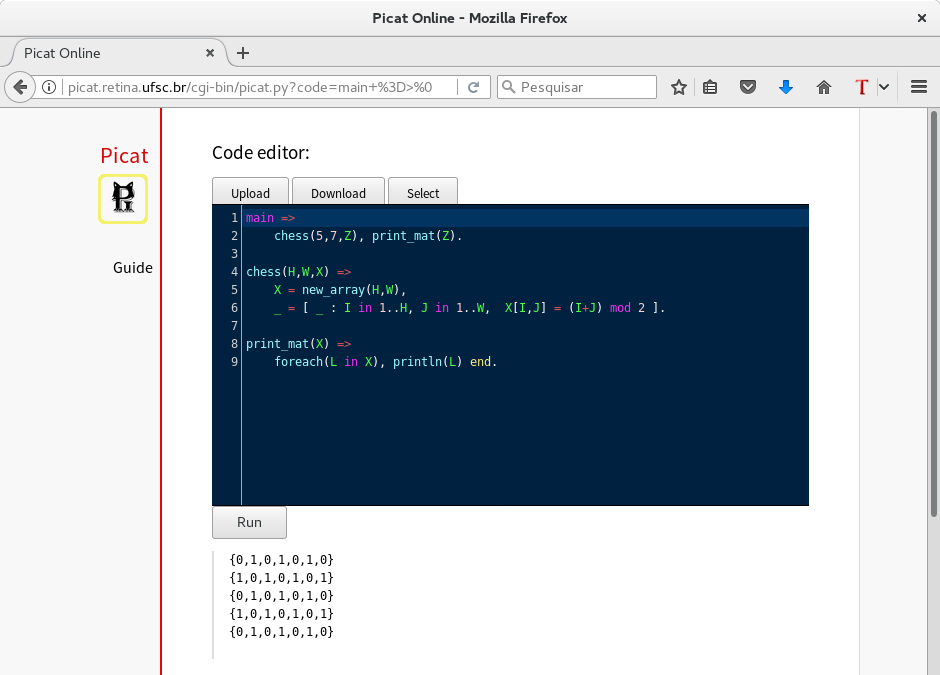
\includegraphics[width=.8\textwidth]{figures/resultado.png}
\end{center}
\end{frame}

%%%%%%%%%%%%%%%%%%%%%%%%%%%%%%%%%%%%%%%%%%%%%%%%%%%%%%%%%%%%%%
\section{Conclusões}


%-------------------------------------------------------------
\begin{frame}

    \frametitle{Conclusões}

    \begin{itemize}
      \item PICAT é recente ... 
      \pause
      \item Uma sintaxe \emph{açucarada}
      \pause
      \item Pontos fortes como: suporte \emph{nativo} a \underline{programação por restrições}, \underline{planejamento} e \underline{programação dinâmica}
      \pause
      \item Uma linguagem em crescimento

      \pause
      \item Um \emph{bom} ambiente de edição de código fonte é um passo-inicial
      
       \pause
      \item Falta integrarmos este editor ao mecanismos de depuração que a linguagem dispõem
      
        \pause
      \item Falta customizarmos \emph{plugins} a editores similares como \emph{geany} e similares, numa versão \emph{off-line}
      
    \end{itemize}
\end{frame}




\end{document}
